\chapter{مسیریابی}\label{ch path planning}

\section{مقدمه}

به طراحی مسیری امن به طوری که برخوردی با موانع پیش نیاید، مسیریابی\LTRfootnote{path planning} می‌گویند. در این پروژه می‌توان مکان ربات‌ها و موانع را به عنوان حالت\LTRfootnote{state} در نظر گرفت. با توجه به اینکه دید از بالا فرض شده است به نحوی که از تمام مکان‌ها اطلاع داشته باشیم، در نتیجه نسبت به تمام موانع اطلاع دقیقی داریم. پس می‌توان گفت در هر حالت نسبت به محیط و داده‌ها به طور کامل مطلع\LTRfootnote{informed} هستیم. در این فصل الگوریتم‌های مسیریابی مبتنی بر روش‌های ابتکاری\LTRfootnote{heuristic} که لازمه آن‌ها مطلع بودن از محیط است، پیاده‌سازی و بررسی گشته‌اند.

\section{الگوریتم‌های ابتکاری}
همانطور که گفته شد، با توجه به شرایط مسئله و مطلع بودن در زمان طراحی مسیر، از الگوریتم‌های ابتکاری استفاده شده است. خصوصیت این الگوریتم‌ها در این است که با ابتکاری که به خرج داده می‌شود، مسئله اندکی ساده‌تر فرض شده و حل می‌گردد. مزیت این الگوریتم‌ها پیچیدگی زمانی کمتر آن‌ها نسبت به مسائلی هستند که مسئله مسیریابی را به طور کامل حل می‌نمایند. این امر در کاربرد رباتیک به دلیل اهمیت بلادرنگ\LTRfootnote{real time} بودن، دارای اهمیت بسیار زیادی می‌باشد. اما همانطور که گفته شد، چون مسئله به طور کامل حل نمی‌گردد، تضمینی برای رسیدن به پاسخ بهینه\LTRfootnote{optimal} وجود ندارد اما پاسخ به طور کلی معقول است، هر چند بهینه نباشد.

برای اعمال این الگوریتم‌ها نیاز به داشتن تعداد حالات محدود بود اما در بازه بین دو عدد متمایز در اعداد حقیقی، مجموعه حالات نامتناهی هستند. لذا از روش نمونه‌برداری\LTRfootnote{sampling based method} استفاده شد. در این پروژه، تمام نقاط با مختصات‌های اعداد صحیح را به عنوان حالت‌ها در نظر گرفتیم. همچنین مجموعه اقدامات\LTRfootnote{actions} به صورت حرکت به حالت‌های مجاور در راستاهای شمال، جنوب، شرق و غرب، و همچنین در راستاهای مورب شمال-غرب، شمال-شرق، جنوب-غرب و جنوب-شرق، تعریف شدند. مسیر خروجی نیز به صورت مجموعه‌ای مرتب از مختصات‌های مجاور که شروع آن مختصات اولیه و پایان آن مختصات نهایی می‌باشد، است. در این پروژه روش‌های ابتکاری \verb|BFS|\LTRfootnote{Breadth-first search}، \verb|search first best Greedy| و $A^*$ پیاده سازی شده‌اند که در ادامه به توضیح آن‌ها می‌پردازیم.

\subsection{الگوریتم $BFS$}
الگوریتم \verb|BFS| در اصل یکی از الگوریتم‌های سرچ معروف و پایه‌ای گراف می‌باشد. برای استفاده از این روش، گراف را به نحوی که هر راس نماینده فقط و فقط یک حالت مجاز، و همچنین هر اقدام نماینده فقط و فقط یک یال باشد ساختیم. همچنین وزن هر یال برابر با نرم-2\LTRfootnote{2-norm} بردار جابه‌جایی اقدام مربوطه، که همان فاصله در مختصات دکارتی است، در نظر گرفته شد. منظور از حالت مجاز، مختصاتی است که در آن مانع نباشد و در محدوده کاری قرار گیرد. حال الگوریتم \verb|BFS| بر روی گراف اعمال می‌شود. قابل ذکر است در صورتی که وزن تمام یال‌ها برابر باشند، اثبات می‌گردد که این الگوریتم به جواب بهین خواهد رسید.

نحوه کار این الگوریتم به این صورت است که با شروع از راس شروع، راس‌های مجاور بررسی می‌شوند و سپس وارد یک صف\LTRfootnote{queue} می‌گردند تا راس‌های مجاور آن‌ها بررسی گردد. صف در ابتدا تنها دارای راس شروع است. برای اینکه راس‌های تکراری وارد صف نگردند، از رنگ‌آمیزی راسی استفاده شد. به این صورت که در ابتدا همه راس‌ها سفید و تنها راس شروع، مشکی می‌باشد. سپس هر راسی که وارد صف می‌شود به رنگ مشکی در می‌آید. در نتیجه هنگام بررسی راس‌های مجاور ابتدا بررسی می‌گردد که چه رنگی دارد. زیرا اگر مشکی باشد یعنی قبلا بررسی شده و دیگر نیازی به بررسی نیست. اینکار تا زمانی که به راس هدف برسیم، ادامه خواهد یافت.

اگر گراف به صورت 
$G = (V, E)$
که در آن \verb|V| مجموعه راس‌ها و \verb|E| مجموعه یال‌ها می‌باشد، تعریف شود، الگوریتم اصلی \verb|BFS| در شکل \ref{Fig BFS Algorithm} به صورت شبه کد آمده است. منظور از نماد \verb|Q| در شبه کد، صف، منظور از \verb|d| فاصله و منظور از $\pi$ والد\LTRfootnote{parent} است. تفاوت در کد ارائه شده در این پروژه با این شبه کد، این است که احتیاجی به رنگ خاکستری نبود و رنگ خاکستری معادل رنگ مشکی در نظر گرفته شد. همچنین چون نقطه هدف داشتیم، در صورتی که به نقطه هدف می‌رسیدیم، حلقه خط 10 شکسته می‌شد و الگوریتم متوقف می‌گشت.
\begin{figure}[!h]
	\centering
	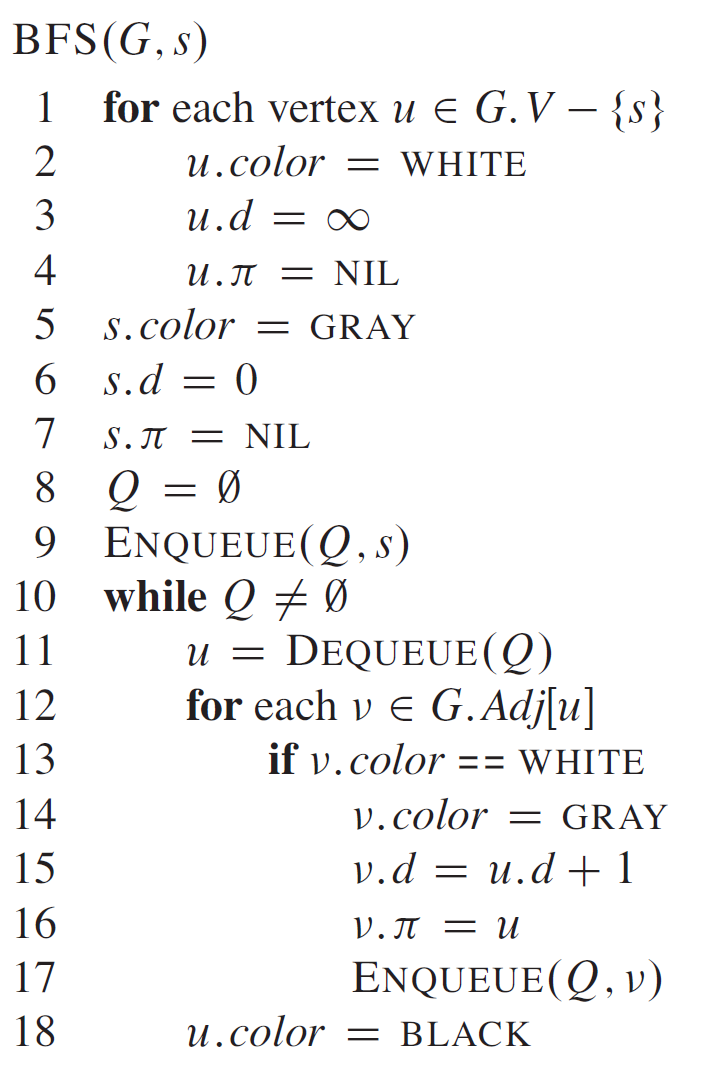
\includegraphics[scale=0.4]{Images/BFS-algorithm.png}
	\caption{شبه کد الگوریتم $BFS$}\label{Fig BFS Algorithm}
\end{figure}

 در شکل \ref{Fig BFS representation} نیز نحوه اعمال شدن الگوریتم \verb|BFS| بر روی یک گراف، نمایش داده شده است.
\begin{figure}[!h]
	\centering
	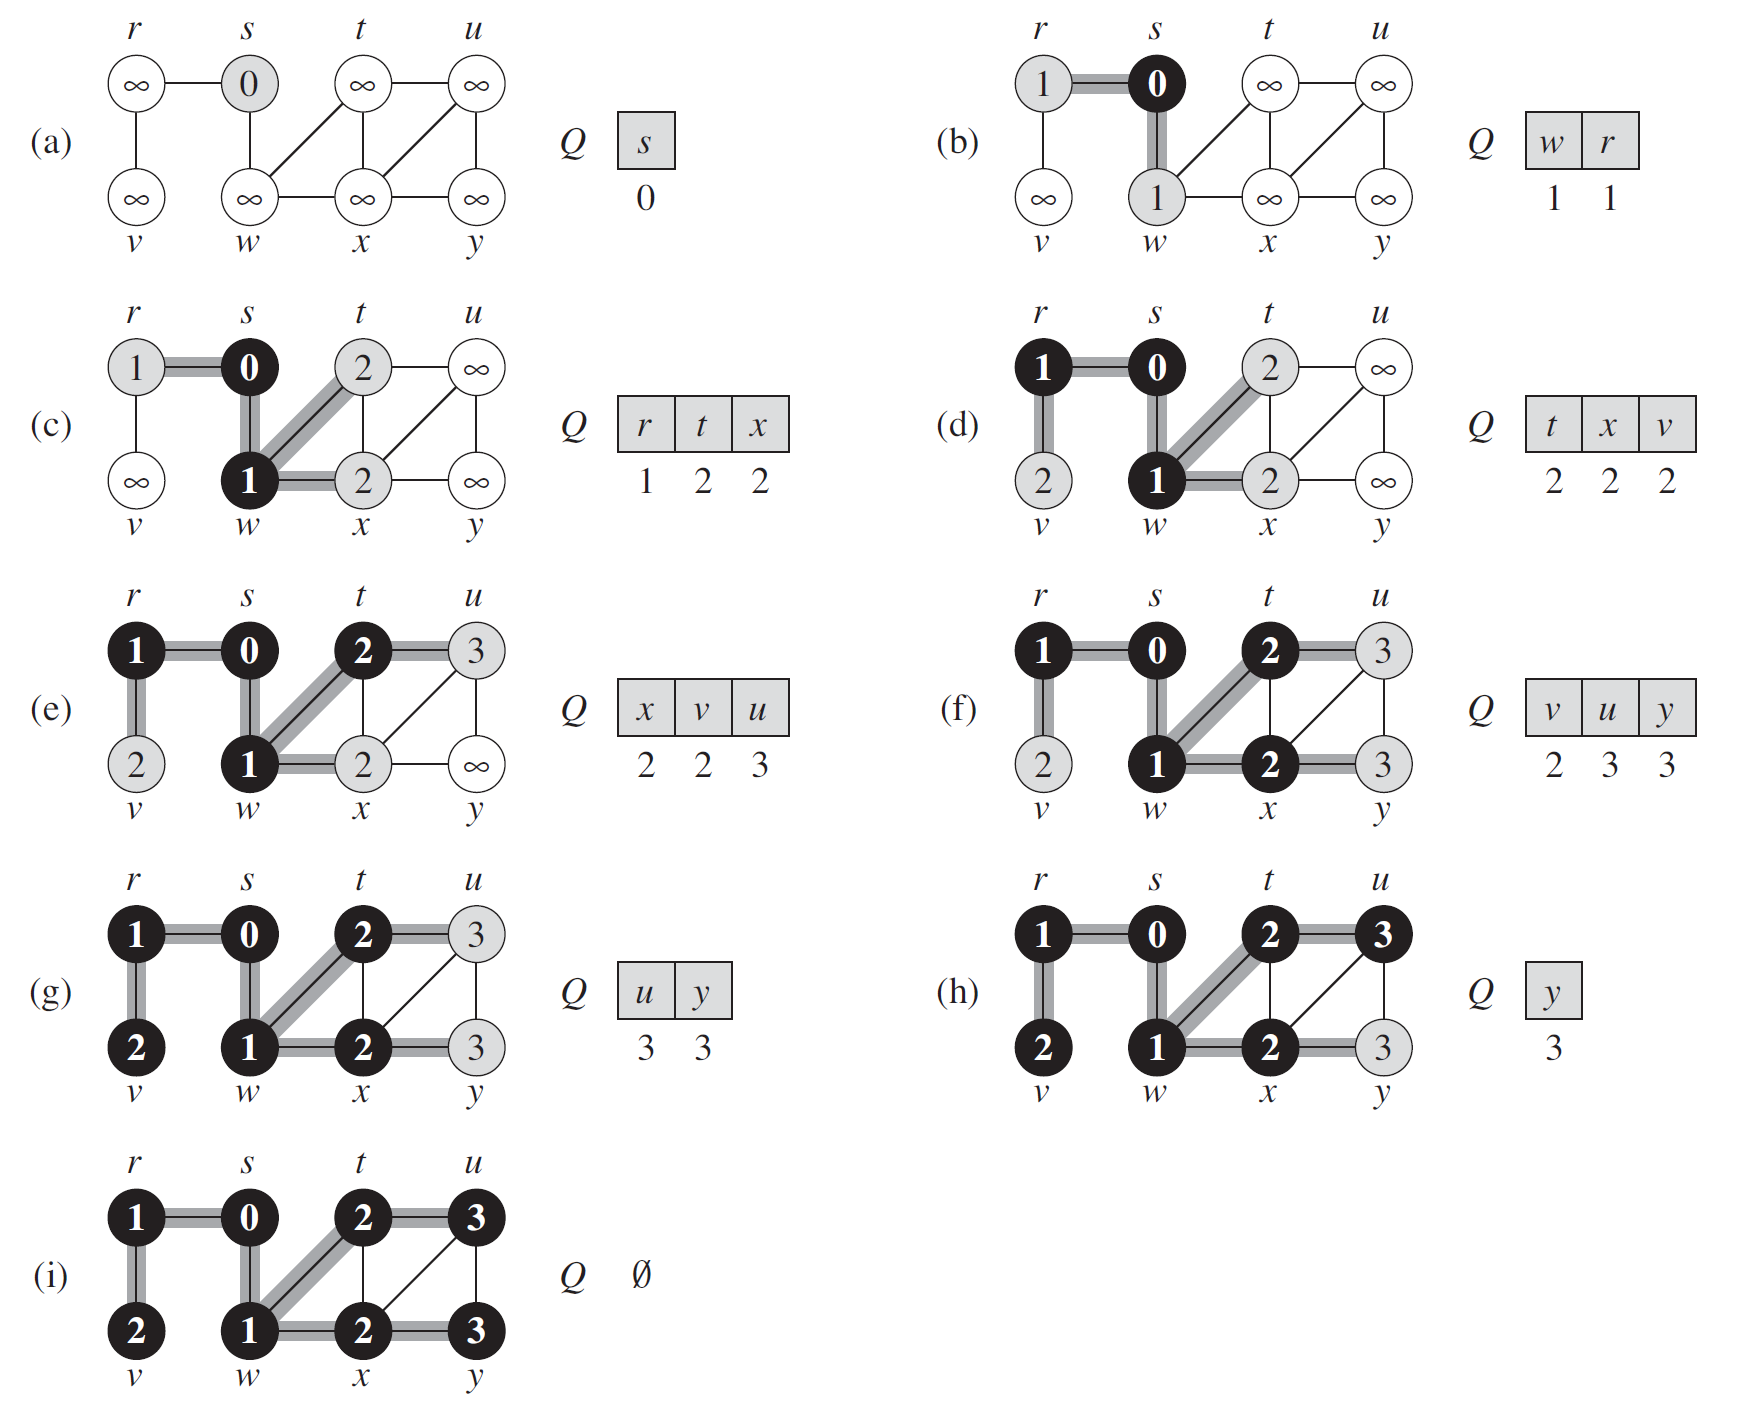
\includegraphics[scale=0.4]{Images/BFS-representation.png}
	\caption{نحوه اعمال شدن الگوریتم $BFS$}\label{Fig BFS representation}
\end{figure}


\newpage
\subsection{الگوریتم $search$ $best-first$ $Greedy$}
ابتکار این روش این است که سعی می‌کند به سمت راسی که کمترین فاصله تا راس هدف دارد، گسترش پیدا کند، به امید آنکه به کوتاه‌ترین مسیر دست یابد. چون کمترین فاصله تا راس هدف را نداریم، حد پایین آن‌ را تقریب می‌زنیم و برابر فاصله قرار می‌دهیم. برای تقریب حد پایین، چون مختصات دو راس را داریم، کافی است طول خط راستی که راس را به راس هدف می‌رساند به دست آورد. در این راستا تابع $h(n)$ برای مختصات راس، \verb|n|، تعریف می‌گردد. اگر مختصات راس هدف با $n^\prime$ نمایش داده شود، مقدار تابع $h(n)$ که طول خط راست از راس تا راس هدف است به صورت زیر تعریف می‌گردد:
\begin{equation}\label{eq heuristic h}
h(n) = \|n - n^\prime\|_2
\end{equation}

مشخصا این روش نیز لزوما به جواب بهین نمی‌رسد، زیرا اصلا می‌تواند بین راسی که انتخاب شده تا راس هدف مسیری نباشد و به بن بست برسیم و مجبور به برگشت باشیم. همچنین برای مثال نقض نیز می‌توان نتیجه این روش را در بخش \ref{sec heuristic result} بررسی کرد که جواب آن بهین نیست.

در هنگام جست‌وجو در هر گام، والد هر راس را در درخت مسیر، به روز می‌گردد و در انتها با کمک از همین والد‌ها و با شروع از راس هدف، تا راس شروع، به عقب برمی‌گردیم. برعکس این مسیر، مسیری خواهد بود که ربات باید بپیماید.

\subsection{الگوریتم $A^*$}
الگوریتم $A^*$ ادامه‌ای بر الگوریتم \verb|search first best Greedy| است که در آن علاوه بر تابع $h(n)$ که در رابطه \ref{eq heuristic h} تعریف شد، تابع $g(n)$ نیز تعریف می‌شود که مسافت واقعی بین نقطه شروع تا راس \verb|n| است. این فواصل با الگوریتم جست‌وجو مرتبا به روز می‌شود و در صورتی که مسیر کوتاه‌تری یافته شود نیز مقادیر آن به همراه مسیر واصله، به روز خواهند شد. همچنین برای یافتن کوتاه‌ترین مسیر نیز همانند الگوریتم \verb|search first best Greedy|، برای هر راس یک والد در نظر گرفته شده است و با پیدا کردن مسیری کوتاه‌تر، مقداری کمتر برای تابع $g(n)$ در راس \verb|n|، والد نیز به راس جدیدی که به آن مسیر دارد، تغییر می‌یابد.

تابعی که طبق آن، راسی که کمترین مقدار آن را داشته باشد جست‌وجو خواهد شد، $f(n)$ می‌نامیم، که به صورت زیر تعریف می‌گردد:
\begin{equation}%\label{eq heuristic f}
	f(n) = g(n) + h(n)
\end{equation}

در نهایت نیز هنگامی که به راس هدف برسیم، الگوریتم جست‌وجو متوقف می‌گردد و سپس به طور بازگشتی از راس هدف، بر روی والدها به عقب برمی‌گردیم تا با عکس کردن جهت حرکت، مسیر ربات تعیین شود. 


\subsection{نتایج و مقایسه الگوریتم‌های ابتکاری}\label{sec heuristic result}
در این قسمت ابتدا به بررسی مسیر یافته شده توسط الگوریتم‌ها پرداخته می‌شود و سپس الگوریتم‌ها از نظر زمانی و ابعاد نقشه، مورد بررسی قرار می‌گیرند.

نقشه مورد استفاده برای بررسی پاسخ‌ها در شکل \ref{Fig mapRooz} آمده است. نقاط مشکی رنگ، مکانی هستند که مانع وجود دارد.
\begin{figure}[!h]
	\centering
	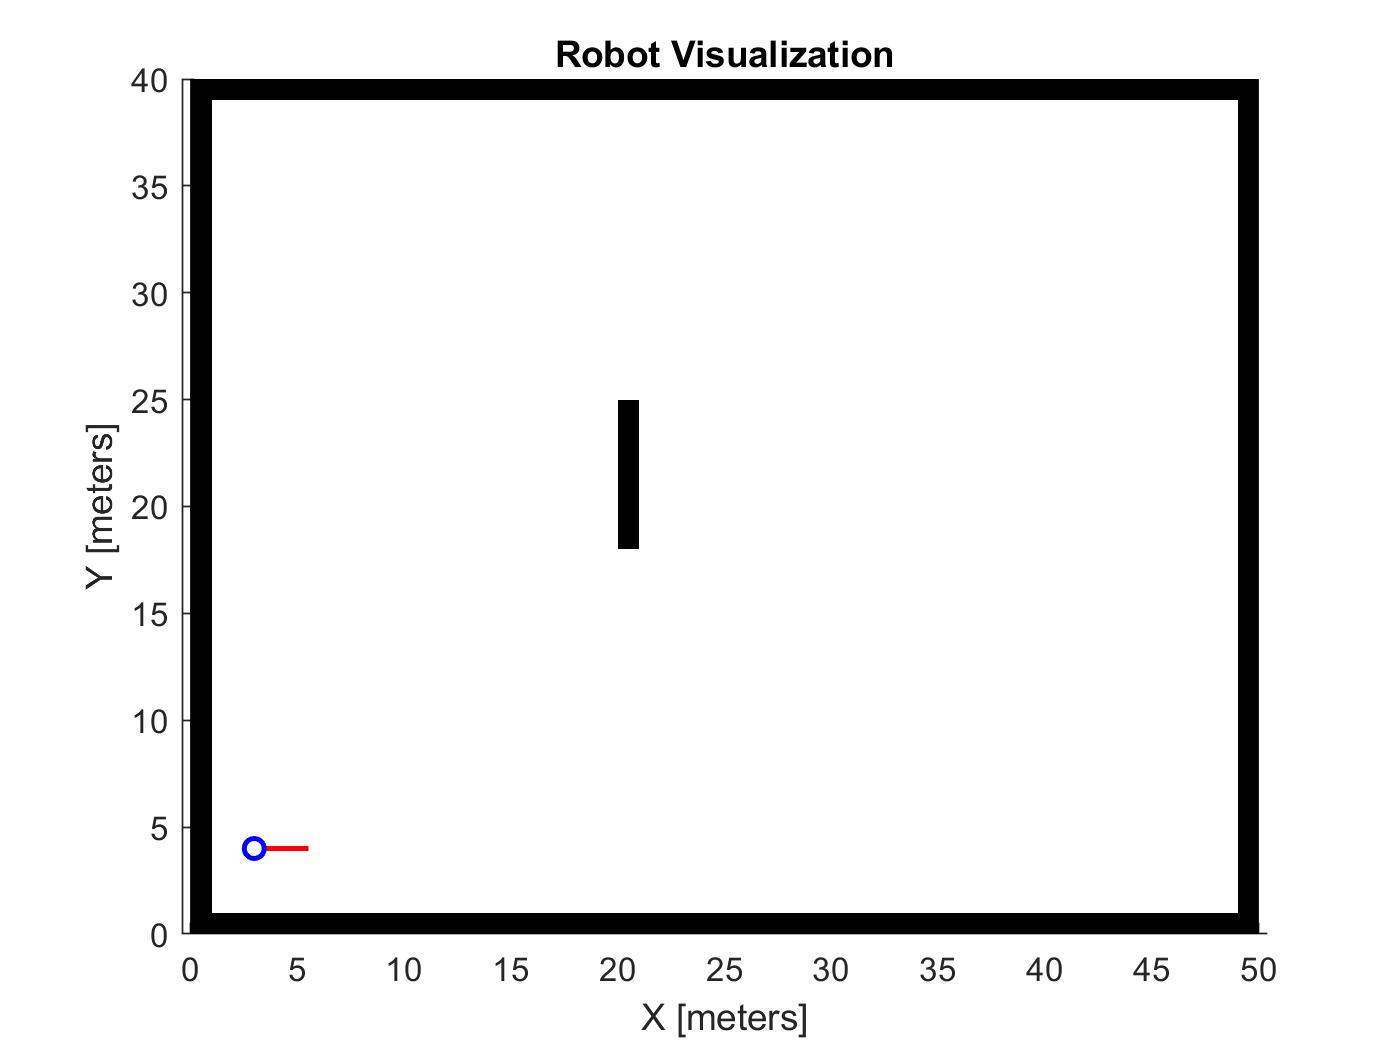
\includegraphics[scale=0.35]{Images/mapRooz.jpg}
	\caption{نقشه‌ای که الگوریتم‌ها به آن اعمال شده‌اند}\label{Fig mapRooz}
\end{figure}

حال برای هر سه الگوریتم، مسیری برای نقطه شروع $[6~~6]^T$ و هدف $[21~~24]^T$ خواسته شد. نتایج به شکل‌های \ref{Fig BFS path}، \ref{Fig Greedy path} و \ref{Fig A-star path} آمده است. نقاط ضربدر خورده قرمز، مسیر الگوریتم، و خط آبی مسیر پیموده شده توسط ربات هستند.
\begin{figure}[!h]
	\centering
	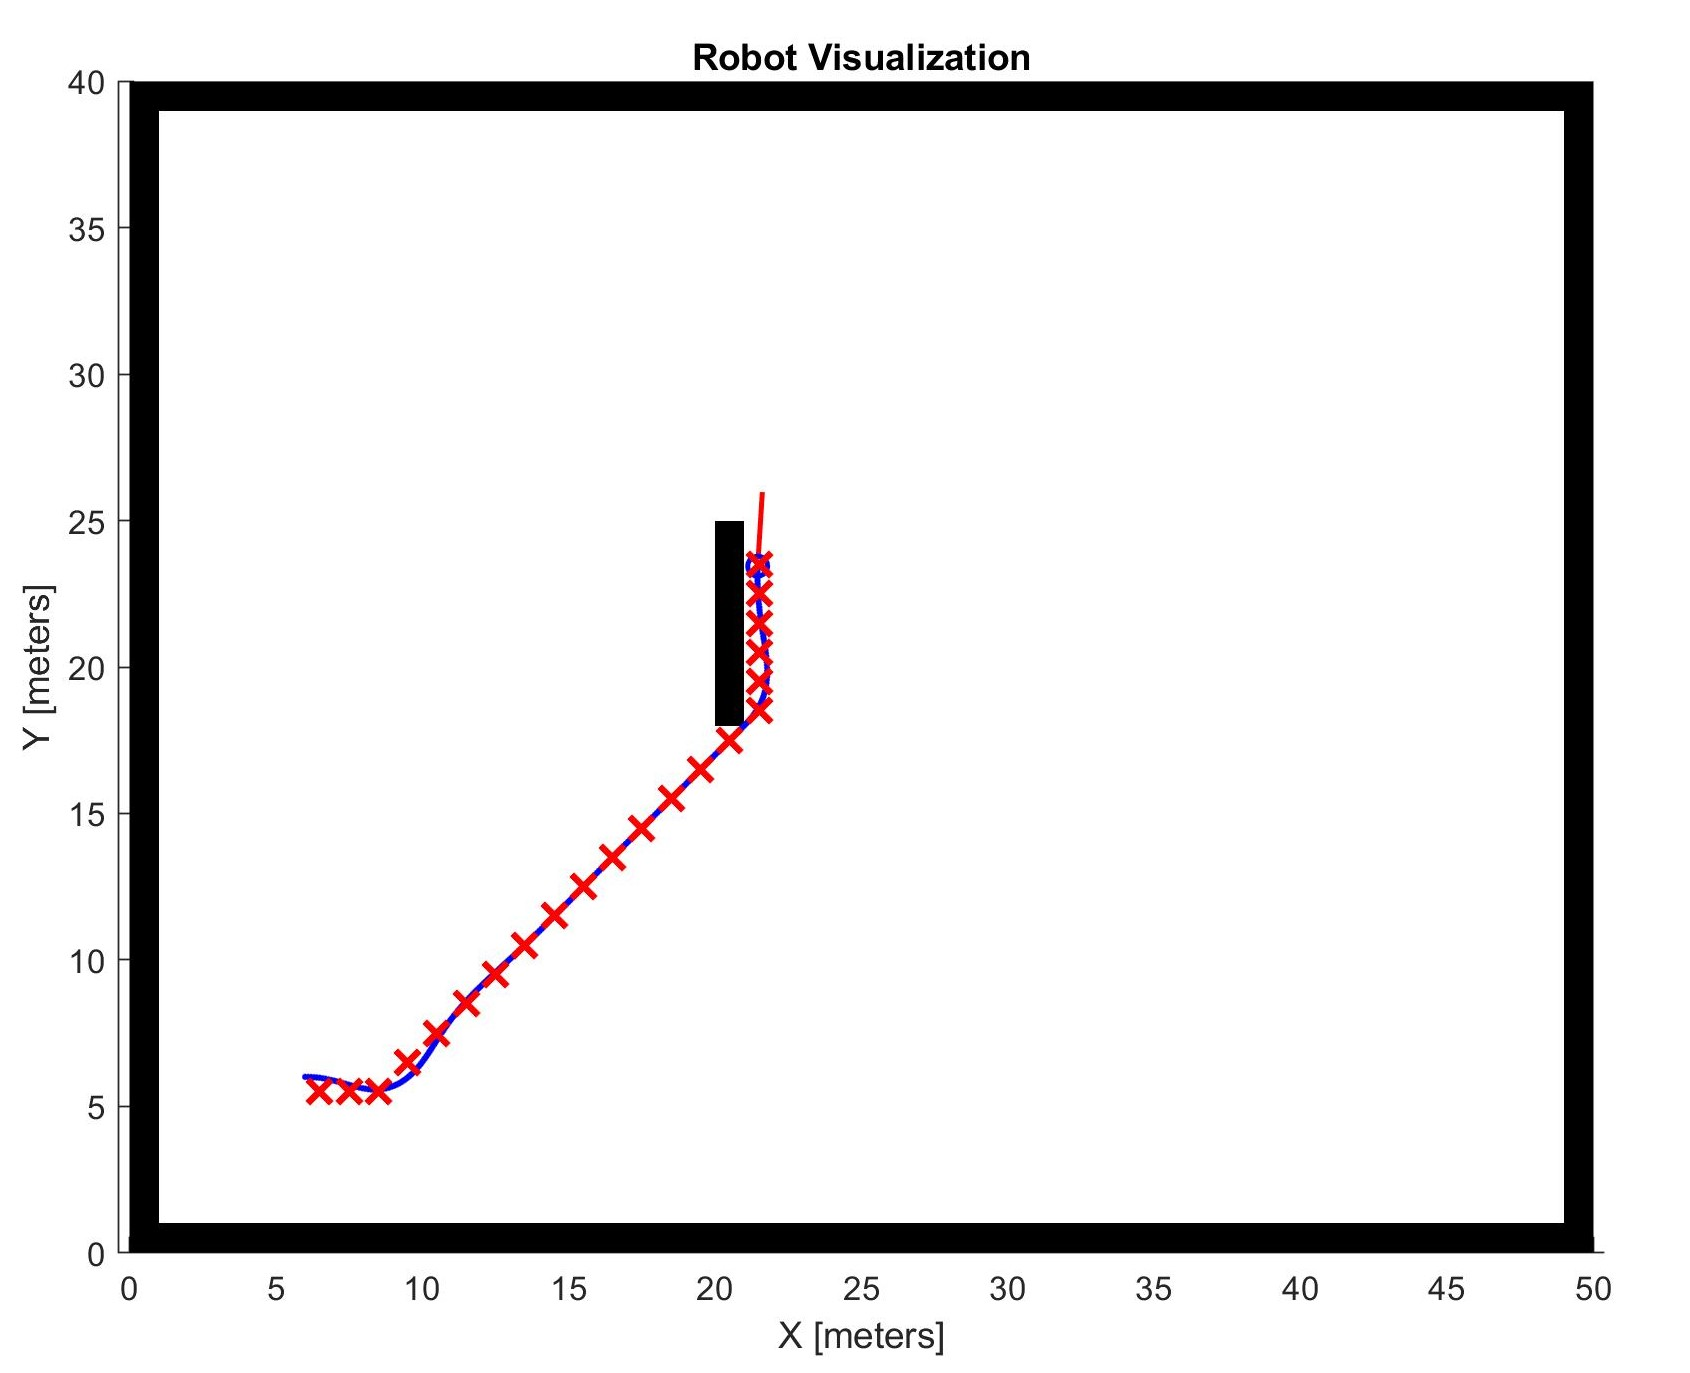
\includegraphics[scale=0.35]{Images/BFS path.jpg}
	\caption{مسیر پیشنهادی توسط الگوریتم $BFS$}\label{Fig BFS path}
\end{figure}

\begin{figure}[!h]
	\centering
	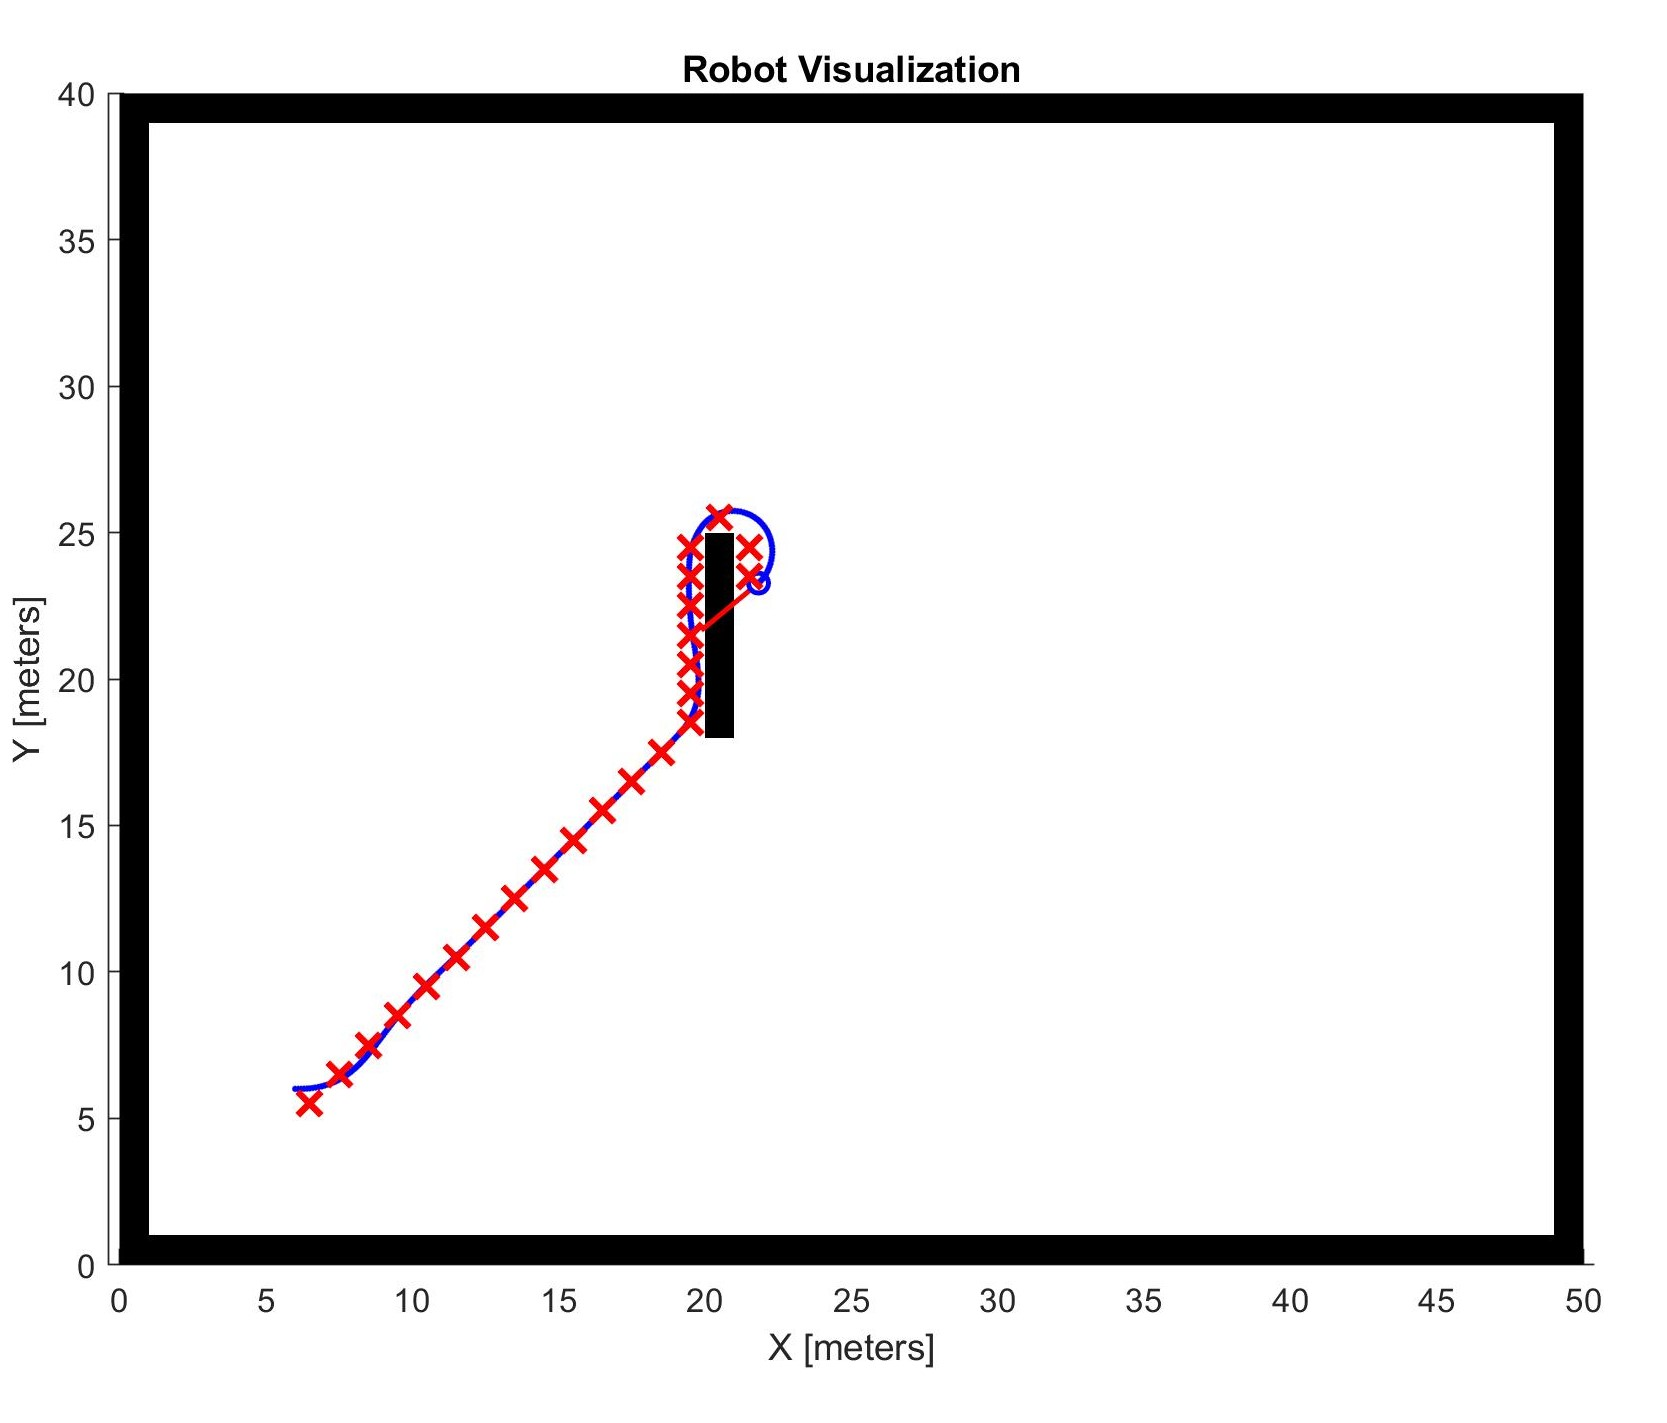
\includegraphics[scale=0.35]{Images/Greedy path.jpg}
	\caption{مسیر پیشنهادی توسط الگوریتم $search$ $best-first$ $Greedy$}\label{Fig Greedy path}
\end{figure}

\begin{figure}[!h]
	\centering
	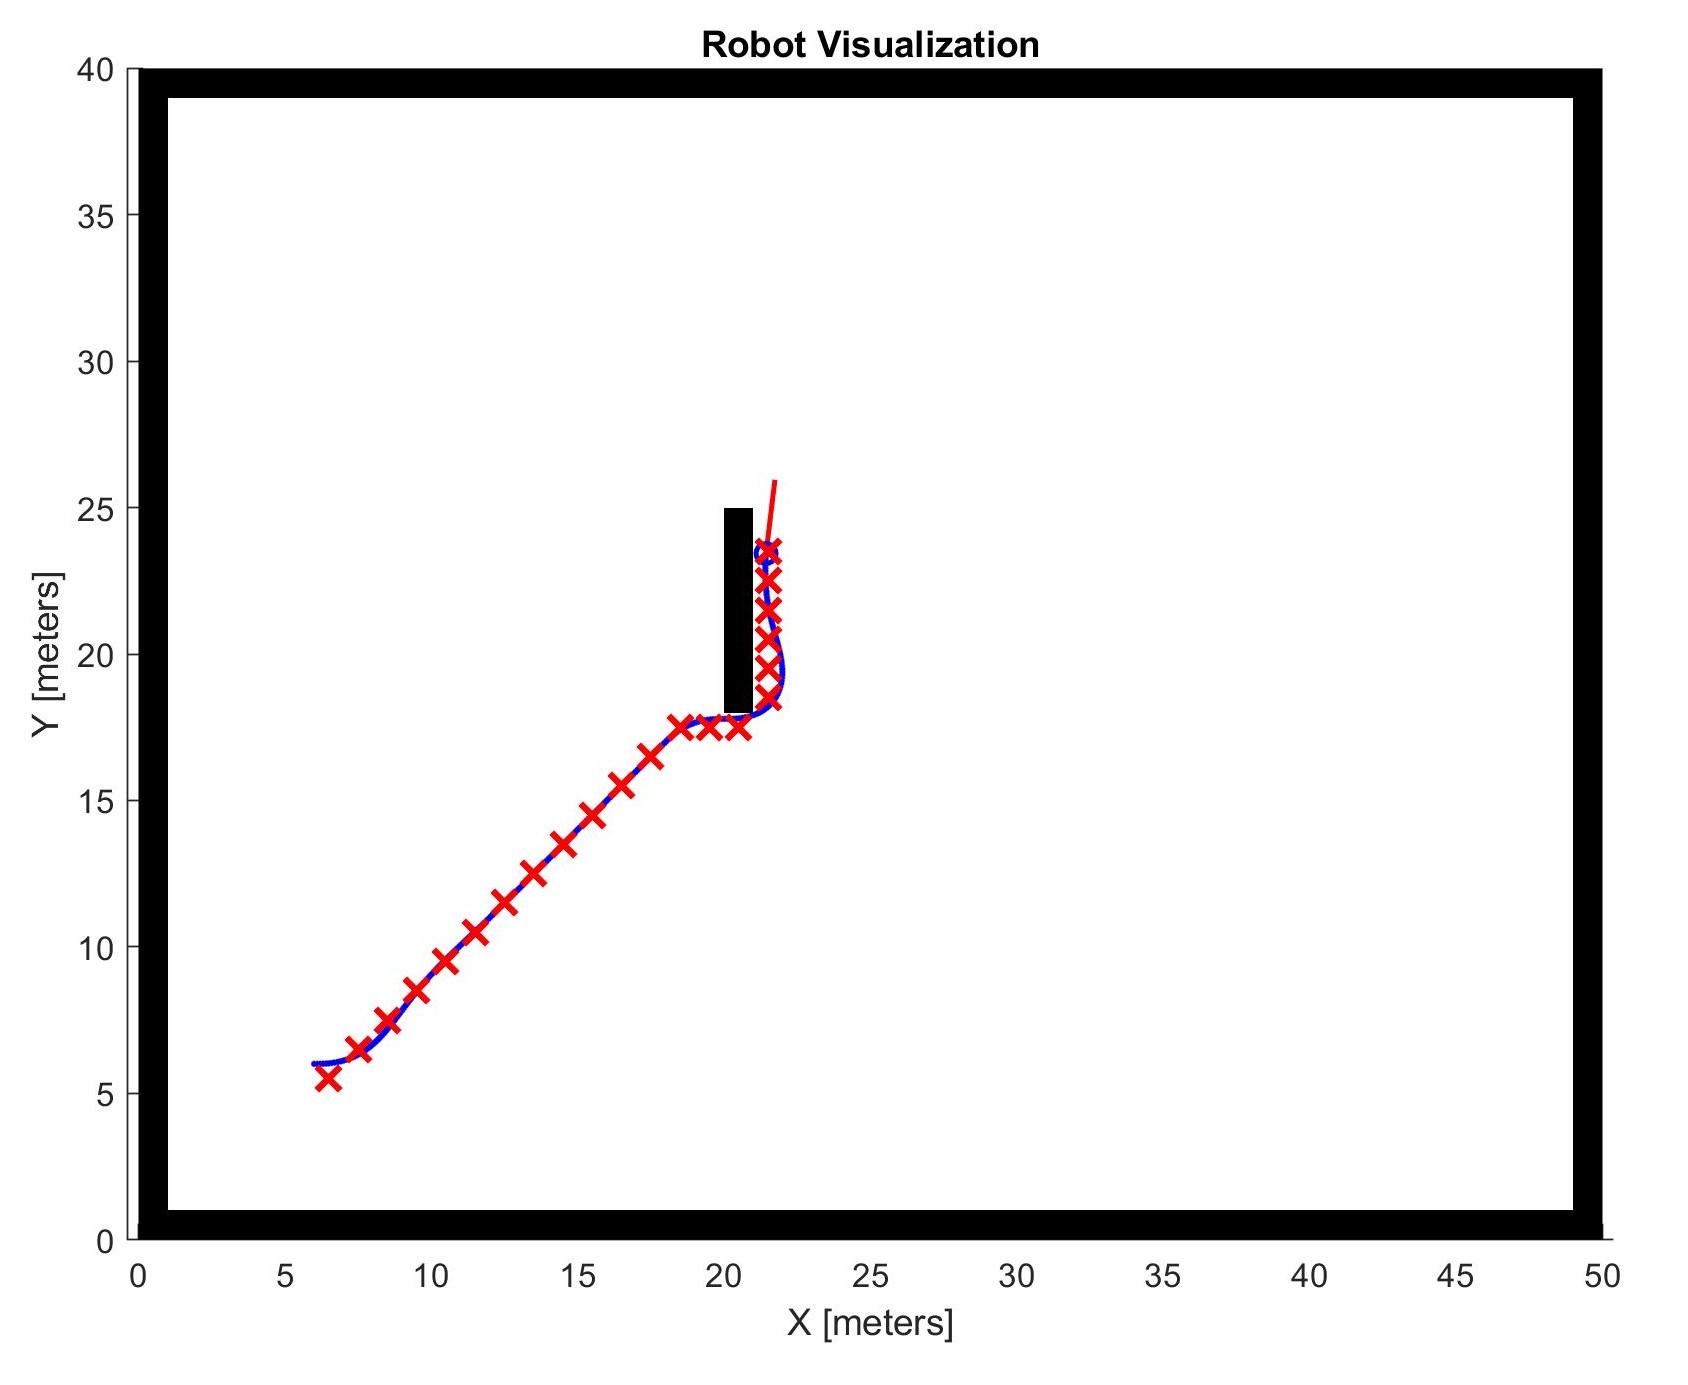
\includegraphics[scale=0.35]{Images/A-star path.jpg}
	\caption{مسیر پیشنهادی توسط الگوریتم $A^*$}\label{Fig A-star path}
\end{figure}

\newpage
همانطور که می‌شود دید در این مثال، الگوریتم، $search$ $best-first$ $Greedy$ مسیر طولانی‌تری نسبت به دو الگوریتم دیگر ارائه داده است. همچنین مسیرهای ارائه شده توسط دو الگوریتم، \verb|BFS| و $A^*$ هر دو بهین هستند.
\newpage
نکته دیگر قابل توجه، این است که هنگام چرخش به خصوص چرخش‌های سنگین همانند برگشت ربات در شکل \ref{Fig Greedy path} در بالای موانع، فشار زیادی به ربات آمده و کنترل مسیر برای او سخت بوده است. در نتیجه بهتر است کنترل‌کننده بهتری برای ربات در نظر گرفته شود. همچنین استفاده از الگوریتم‌هایی که سعی کنند میزان فشار وارده بر ربات را در تصمیمشان در نظر گرفته و کاهش دهند نیز، می‌تواند عضو کارهای آینده باشد.
\newpage
حال نوبت بررسی زمان مورد نیاز برای اجرای هر الگوریتم است. در این راستا، سه الگوریتم با نقاط تصادفی شروع و هدف، در حالی که برای هر سه یکسان باشند، اجرا گشتند. به ازای هر اندازه، 100 بار الگوریتم‌ها برای نقاط متفاوت بررسی و سپس از زمان آن‌ها میانگین گرفته شد. نتیجه در شکل \ref{Fig heuristic time} به نمایش در آمده است. همانطور که مشاهده می‌شود، زمان الگوریتم $A^*$ به مراتب بیشتر از الگوریتم‌های دیگر است. همچنین الگوریتم $search$ $best-first$ $Greedy$ کمترین زمان را دارد. در نتیجه هر چقدر بخواهیم به جواب معقولتری برسیم، مدت زمان بیشتر مورد نیاز است. در حالت کلی با توجه به اینکه برای 35000 نود، در کمتر از 200 میلی‌ثانیه برای الگوریتم $A^*$ به جواب رسیده است، استفاده از این الگوریتم توصیه می‌شود. قابل ذکر است که الگوریتم $A^*$ روش معقول‌تری نسبت به دو الگوریتم دیگر دارد و همچنین عملکرد آن در شرایطی که وزن‌ یال‌ها نسبت به هم بسیار متفاوت باشند بهتر نیز خواهد بود و قابلیت تعمیم به مسائل دیگر را نیز دارد.

\begin{figure}[!h]
	\centering
	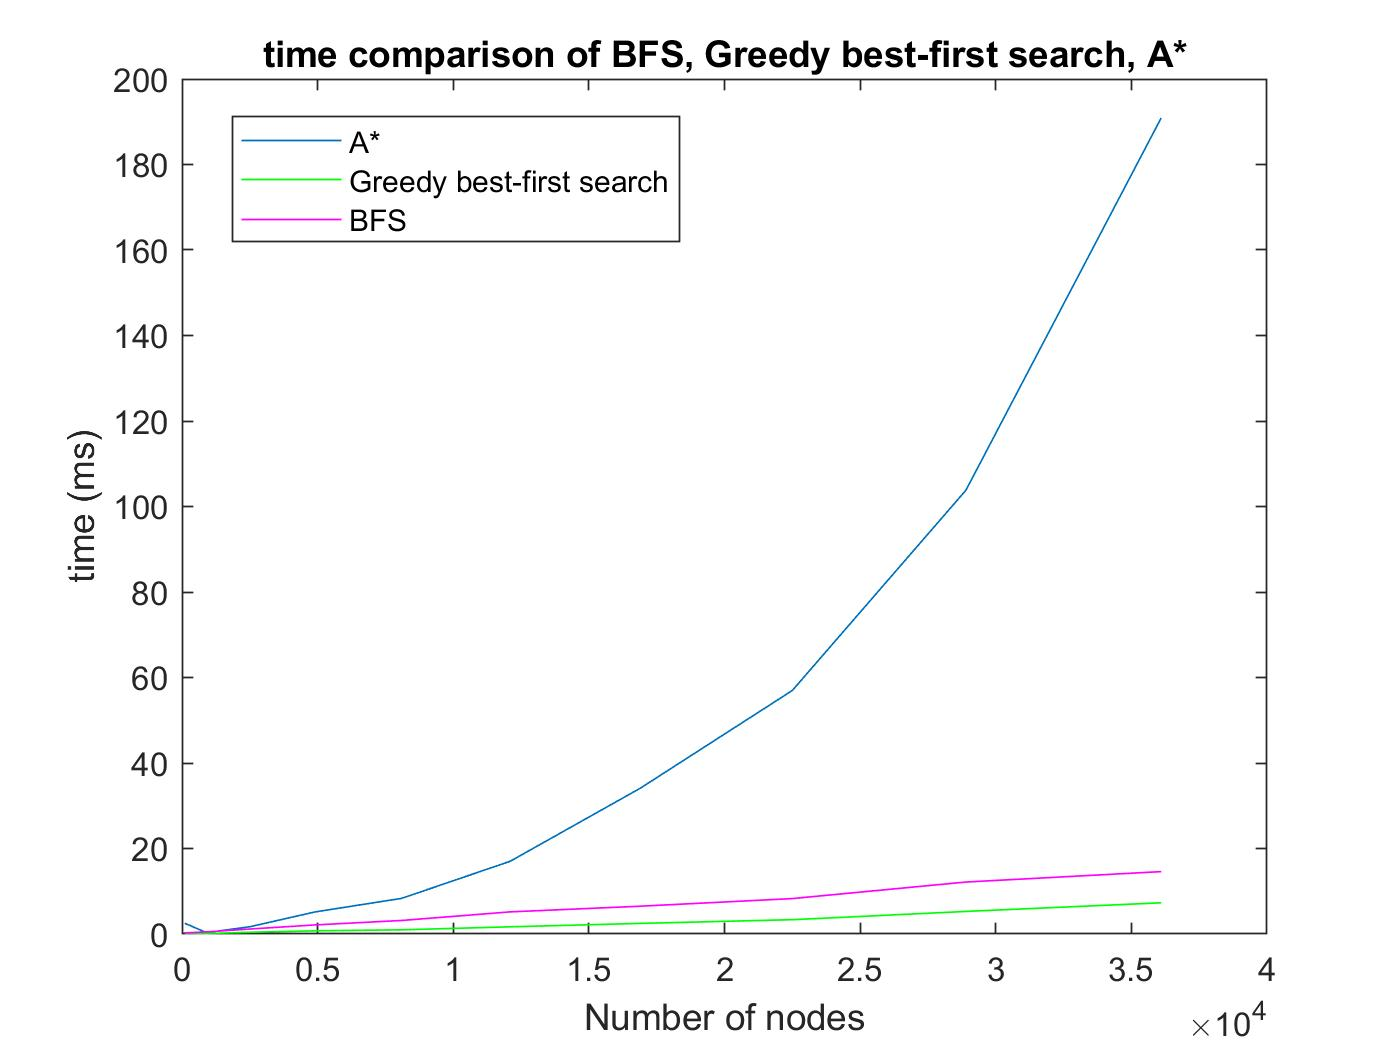
\includegraphics[scale=0.35]{Images/Heuristic time.jpg}
	\caption{مقایسه زمانی سه الگوریتم $BFS$، $search$ $best-first$ $Greedy$ و $A^*$}\label{Fig heuristic time}
\end{figure}





















